% Source: TeX Live PGF manual, pgfmanual-en-library-3d.tex.
\documentclass[border=2pt]{standalone}
\usepackage{tikz}
\usetikzlibrary{3d}

\begin{document}
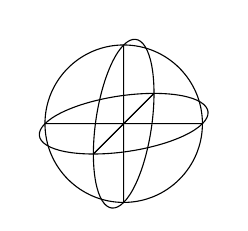
\begin{tikzpicture}
  \begin{scope}[canvas is zy plane at x=0]
    \draw (0,0) circle (1cm);
    \draw (-1,0) -- (1,0) (0,-1) -- (0,1);
  \end{scope}

  \begin{scope}[canvas is zx plane at y=0]
    \draw (0,0) circle (1cm);
    \draw (-1,0) -- (1,0) (0,-1) -- (0,1);
  \end{scope}

  \begin{scope}[canvas is xy plane at z=0]
    \draw (0,0) circle (1cm);
    \draw (-1,0) -- (1,0) (0,-1) -- (0,1);
  \end{scope}
\end{tikzpicture}
\end{document}
